\documentclass[10pt,onecolumn,letterpaper]{article}

% tikz
\usepackage{tikz}
\usetikzlibrary{intersections, angles, quotes, positioning}
\usetikzlibrary{arrows.meta}
\usepackage{pgfplots}
\pgfplotsset{compat=1.13}


\tikzset{
	force/.style={thick, {Circle[length=2pt]}-stealth, shorten <=-1pt}
}


% quiver style
\usepackage{tikz-cd}
% `calc` is necessary to draw curved arrows.
\usetikzlibrary{calc}
% `pathmorphing` is necessary to draw squiggly arrows.
\usetikzlibrary{decorations.pathmorphing}

% A TikZ style for curved arrows of a fixed height, due to AndréC.
\tikzset{curve/.style={settings={#1},to path={(\tikztostart)
                .. controls ($(\tikztostart)!\pv{pos}!(\tikztotarget)!\pv{height}!270:(\tikztotarget)$)
                and ($(\tikztostart)!1-\pv{pos}!(\tikztotarget)!\pv{height}!270:(\tikztotarget)$)
                .. (\tikztotarget)\tikztonodes}},
settings/.code={\tikzset{quiver/.cd,#1}
        \def\pv##1{\pgfkeysvalueof{/tikz/quiver/##1}}},
quiver/.cd,pos/.initial=0.35,height/.initial=0}

% TikZ arrowhead/tail styles.
\tikzset{tail reversed/.code={\pgfsetarrowsstart{tikzcd to}}}
\tikzset{2tail/.code={\pgfsetarrowsstart{Implies[reversed]}}}
\tikzset{2tail reversed/.code={\pgfsetarrowsstart{Implies}}}
% TikZ arrow styles.
\tikzset{no body/.style={/tikz/dash pattern=on 0 off 1mm}}

\usepackage{iccv}
\usepackage{times}
\usepackage{epsfig}
\usepackage{graphicx}
\usepackage{amsmath}
\usepackage{amssymb}
\usepackage{amsthm}
\usepackage{gensymb}
\usepackage{ctable}
\usepackage{esvect}
\usepackage{array}
\usepackage{enumitem}
% \usepackage{hyperref}

\usepackage{algorithm}
\usepackage{algpseudocode}


\newcolumntype{C}[1]{>{\centering\let\newline\\\arraybackslash\hspace{0pt}}m{#1}}

% Include other packages here, before hyperref.

% If you comment hyperref and then uncomment it, you should delete
% egpaper.aux before re-running latex.  (Or just hit 'q' on the first latex
% run, let it finish, and you should be clear).
\usepackage[breaklinks=true,bookmarks=false]{hyperref}

\iccvfinalcopy % *** Uncomment this line for the final submission

% \def\iccvPaperID{1566880001704} % *** Enter the ICCV Paper ID here
\def\httilde{\mbox{\tt\raisebox{-.5ex}{\symbol{126}}}}

% Pages are numbered in submission mode, and unnumbered in camera-ready
% \ificcvfinal\pagestyle{empty}\fi

\newtheorem{thm}{Theorem}[section]
\newtheorem{ithm}{Theorem}
\newtheorem{icor}[ithm]{Corollary}
\newtheorem{lem}[thm]{Lemma}
\newtheorem{conj}[thm]{Conjecture}
\newtheorem{obs}[thm]{Observation}
\newtheorem{remark}[thm]{Remark}
\newtheorem{prop}[thm]{Proposition}
\newtheorem{cor}[thm]{Corollary}
\newtheorem{claim}[thm]{Claim}
\newtheorem{problem}{Problem}

\newtheorem{defin}[thm]{Definition}
\newtheorem{example}[thm]{Example}
\newtheorem{assumption}[thm]{Assumption}
\newtheorem{exercise}[thm]{Exercise}
\renewcommand*{\proofname}{{\color{blue}Proof}}

\newcommand{\cc}{\mathbb{C}}
\newcommand{\ee}{\mathbb{E}}
\newcommand{\ff}{\mathbb{F}}
\renewcommand{\gg}{\mathbb{G}}
\newcommand{\hh}{\mathbb{H}}
\newcommand{\nn}{\mathbb{N}}
\newcommand{\pp}{\mathbb{P}}
\newcommand{\qq}{\mathbb{Q}}
\newcommand{\rr}{\mathbb{R}}
\newcommand{\zz}{\mathbb{Z}}
\newcommand{\Var}{\mathrm{Var}}

\renewenvironment{abstract}
{\begin{center}\begin{minipage}{0.7\textwidth} % Adjust the 0.8 to make it smaller or larger
\small\textbf{Abstract}\par\medskip\noindent}
{\end{minipage}\end{center}}

\newcommand{\eps}{\varepsilon}
\let\epsilon\varepsilon

\newcommand{\erdos}{Erdös-Rényi }

\begin{document}

%%%%%%%%% TITLE
\title{Robust Estimation for the \erdos Model}

\author{Heon Lee, George Chemmala, Arjan Chakravarthy\\
Brown University\\
{\tt\small heon\_lee@brown.edu}
{\tt\small george\_chemmala@brown.edu}
{\tt\small arjan\_chakravarthy@brown.edu}
% For a paper whose authors are all at the same institution,
% omit the following lines up until the closing ``}''.
% Additional authors and addresses can be added with ``\and'',
% just like the second author.
% To save space, use either the email address or home page, not both
}


\maketitle

% \ificcvfinal\thispagestyle{empty}\fi

%%%%%%%%% ABSTRACT
\begin{abstract}
We study the robust estimation of the edge probability $p$ in the \erdos random graph model under adversarial perturbation of vertices. We define a new class of adversarial models, the $(q,\eps)$-adversarial model, which naturally generalizes to corresponding definitions for $(q,\eps)$-oblivious and $(q,\eps)$-omniscient adversaries, analogous to the $\eps$-adversarial framework. This new model allows us to explore robustness across varying levels of adversarial strengths while maintaining a unified framework for analysis.

In the presence of a $(q,\epsilon)$-oblivious adversary, we propose a novel algorithm that runs in $O(n)$ time and guarantees $|p - \hat p| \leq O(1/\sqrt[4]{n})$ with probability at least $1-\frac{1}{\sqrt{n}}$, representing a significant improvement in both efficiency and accuracy compared to existing methods designed for $\eps$-omniscient adversaries. Existing methods either have a slower runtime with a comparable error guarantee or a similar runtime with a worse error guarantee. Furthermore, we introduce an iterative algorithm that uses variance-based filtering to identify and remove corrupted vertices. This approach empirically demonstrates strong performance and achieves a runtime of $O(\eps n^3)$. Work is ongoing to establish theoretical guarantees for this method.
\end{abstract}

%%%%%%%%% BODY TEXT
\section{Introduction}
% why robustness is important
The \erdos graph model is a fundamental framework in network theory and probability, commonly used for studying random graphs \cite{Albert_2002}. It is constructed by independently connecting each pair of $n$ vertices with probability $p$ \cite{Erds2022}. Despite its simplicity and inability to fully represent the complexity of real-world networks, the \erdos model serves as a foundational tool for analyzing network properties. Applications span various domains, including social, biological, and communication networks \cite{Albert_2002}. This paper investigates a scenario where an adversary corrupts an $\eps$-fraction of the vertices in an \erdos graph. The objective is to estimate the original edge formation probability $p$ given the corrupted graph.

\subsection{Problem Setup}
In this paper, we are primarily concerned with the \erdos random graph model which was first formally defined by Edgar Gilbert in 1959 and independently rediscovered by its namesakes Erdös and Rényi later that year \cite{Erds2022} \cite{Gilbert1959}. Notice that the $p$ value of the \erdos graph has a direct impact on the degree distribution of the graph which follows a Binomial distribution $B(n - 1,p)$ \cite{Newman2001}. The expected degree of any given vertex in the graph is $(n-1)p$, since each vertex is connected to $n - 1$ other vertices with probability $p$.

Refer to Figure \ref{erdos-renyi example} for an example of an \erdos graph with $n=10$ vertices and $p= 1 / 2$. 
\begin{defin}
  \label{\erdos Graph}
  The \erdos random graph model $G(n,p)$ is a probability distribution over graphs with $n$ vertices, where each edge is included independently with probability $p$.
\end{defin}

\begin{figure}[ht]
\centering
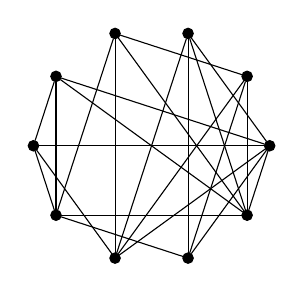
\begin{tikzpicture}[scale=.75]
  \foreach \i in {1,...,10} {
    \node[circle, draw, fill=black, scale=.4] (N\i) at ({360/10 * (\i - 1)}:2) {};
  }
  \foreach \i in {1,...,10} {
    \foreach \j in {\i,...,10} {
      \ifnum\i=\j\relax\else
      \pgfmathparse{int(rnd < 0.5)}
      \ifnum\pgfmathresult=1
      \draw (N\i) -- (N\j);
      \fi
      \fi
    }
  }
\end{tikzpicture}
\caption{Example of an \erdos graph $G(10, 1 / 2)$}
\label{erdos-renyi example}
\end{figure}

The central challenge of this paper is to estimate the true edge probability $p$ of a graph \(G \sim G(n, p)\) in the presence of adversarial corruption. Specifically, we consider an adversary
\(\mathcal{A}\) capable of corrupting up to an $\eps$-fraction of the vertices and producing a corrupted graph, \(\mathcal{A}(G)\). The adversary can alter the structure of the graph by modifying any edge that is incident to a corrupted vertex, including both adding and removing an edge.

With this setup, we build on two $\eps$-adversaries proposed by Acharya, Jain, Kamath, Suresh, and Zhang
\cite{acharya2022robustestimationrandomgraphs} with our own $(q, \eps)$-adversary. 
\begin{enumerate}[align=left]
  \item[\emph{$\eps$-omniscient adversary}:] The adversary knows the true value of the edge probability \(p\) and observes the realization of the graph \(G \sim G(n, p)\). They then choose the set of corrupted vertices and rewire the edges of these corrupted vertices.
  \item[\emph{$\eps$-oblivious adversary}:] The adversary knows the true value of the edge probability \(p\). They must choose the set of corrupted vertices and the distribution of edges of the corrupted vertices without the realization of the graph \(G\).
  \item[\emph{$(q, \eps)$-omniscient adversary}:] The adversary knows the true value of the edge probability \(p\) and observes the realization of the graph $G\sim G(n,p)$. They then choose the set of corrupted vertices, and the edges of the corrupted vertices are rewired with a new edge probability \(q\).
  \item[\emph{$(q, \eps)$-oblivious adversary}:] The adversary knows the true value of the edge probability \(p\). They must choose the set of corrupted vertices and the distribution of edges of the corrupted vertices without the realization \(G\). However, the adversary can choose to rewire the edges adjacent to the corrupted vertices with a new edge probability \(q\).
\end{enumerate}

Despite this adversarial perturbation, we aim to estimate the true edge probability \(p\). While this might initially seem straightforward, given that the adversary is limited to corrupting an $\eps$-fraction of corrupted vertices, the impact is more complex. Specifically, corrupting a single vertex alters the degree distribution of the uncorrupted vertices. In other words, when the adversary perturbs the edges connected to corrupted vertices, it indirectly creates or removes edges incident to uncorrupted vertices as well. Consequently, the observed $p$ value in the corrupted graph can deviate significantly from the true $p$ value of the original graph prior to corruption.

The primary metric we seek to optimize is $$|p - \hat p|,$$ the difference between the theoretical $p$ value of the graph and the robust estimation on the corrupted graph, $\hat{p}$.

\subsection{Related Work}
% Robust Statistics

% Stochastic block model
On our particular problem, we examined a paper by Acharya, Jain, Kamath, Suresh, and Zhang \cite{acharya2022robustestimationrandomgraphs} that introduced the $\eps$-omniscient adversary and proposed the naive mean, naive median, the Prune algorithms, for both the mean and the median, and the Spectral algorithm. 

The naive mean and median algorithms estimate the edge probability $p$ using the degree distribution of the corrupted graph. In an uncorrupted graph, the mean and median degrees of the vertices are expected to be $(n-1)p$. The naive algorithm calculates the mean or median degree of the vertices in the corrupted graph and normalizes this value by dividing it by $(n-1)$, yielding an estimate for $p$.

The Prune algorithm removes an $\eps$-fraction of the vertices from the top and bottom of the degree distribution---the extremal vertex degrees---and then estimates the edge probability $p$ based on the remaining vertices with the mean and median of the pruned degree distribution. By removing the extremal vertex degrees, Acharya et.al proves that the pruned mean would have an error proportional to $O(\eps^2)$ and the pruned median would have an error proportional to $O(\eps)$. The algorithm has a runtime of $O(n \log (n\eps))$ to find the $\eps$-fraction of vertices with the highest and lowest degrees \cite{acharya2022robustestimationrandomgraphs}.

The Spectral algorithm is based on the fact that the metric \(\| (A - p_S)_{S \times S}\|_2\) is small for when \(S\) is a set of uncorrupted vertices. Here \(p_S:=(\sum_{i,j\in S}A_{i,j})/{|S|^2}\); this is the measured \(p\) value of the sub-graph \(G_S\)---the graph that consists of vertices in \(S\). Intuitively, this metric should be small for uncorrupted subsets because the expected value of the entries of the adjacency matrix is \(p\) for uncorrupted vertices. The Spectral algorithm estimates the edge probability \(p\) by minimizing this norm by removing vertices in \(S\) that contribute to increasing this norm. We can find these vertices by computing the top eigenvector of \((A - p_S)\). Eventually, we will get a set of vertices that appear to be uncorrupted and estimate the edge probability \(p\) based on the mean of the degree distribution of these vertices. 

\subsection{Contributions}
This paper introduces the $(q, \eps)$-adversarial model, extending the $\eps$-adversarial framework to encompass varying levels of adversarial strength under a unified analysis. We propose three robust algorithms for estimating the edge probability \( p \): the Mean-Adjusted Median, the Bias-Corrected Mean-Adjusted Median, and the Variance-Based Filtering method. Our contributions include:\begin{enumerate}
    \item Developing a novel Mean-Adjusted Median algorithm with a runtime of \( O(n) \) and theoretical guarantees on its error bound.
    \item Enhancing the Mean-Adjusted Median with a Bias-Correction mechanism, leading to improved accuracy.
    \item Designing a Variance-Based Filtering algorithm for identifying corrupted vertices, supported by empirical evidence.
\end{enumerate}

\section{Notation}
\begin{enumerate}[align=left]
  \item[\(G(n, p)\):] \erdos random model with \(n\) vertices and edge probability \(p\).
  \item[\(\mathcal{A}(G)\):] Perturbed graph with a fraction \(\eps\) of corrupted vertices.
  % \item[\(F\):] Set of uncorrupted vertices.
  % \item[\(D\):] Degree distribution of the graph.
  % \item[\(D'\):] Degree distribution of the perturbed graph.
  \item[\(\bar{p}\) and \(\tilde{p}\):] Normalized mean and median of the degree distribution.
  \item[\(\bar{d}\) and \(\tilde{d}\):] Mean and median of the degree distribution.
  \item[\(s^2\):] Variance of the degrees of the graph.
  \item[\(\hat{\sigma}^2\):] Variance of the degrees of the perturbed graph.
  \item[\(\deg(v)\):] Degree of vertex \(v\)
\end{enumerate}

\section{Mean-Adjusted Median}
In this section, we propose an algorithm based on the median and mean of the degree distribution for robustly estimating the edge probability $p$. Since the median is more robust to outliers than the mean for $(q,\eps)$-oblivious adversary, the perturbed median of the degree distribution consistently tends closer to the median of the distribution prior to adversarial corruption than the corresponding mean values. Thus, we derive our Mean-Adjusted Median algorithm by analyzing this difference between the median and the mean.

Plotting out a histogram (Figure \ref{fig:mean-vs-median}) of the degree distribution of the graph altered by the \((q,\eps)\)-adversary, we can see that the median of the degree distribution is roughly two times closer to the mean of the original degree distribution than the mean. Since the mean of the original degree distribution is \((n-1)p\), in order to derive $\hat{p}$, we divide an estimator of the original degree distribution by a factor of \(n-1\). This leads us to consider using the difference between the mean and the median in order to find \(p\).

\begin{figure}[hb]
    \centering
    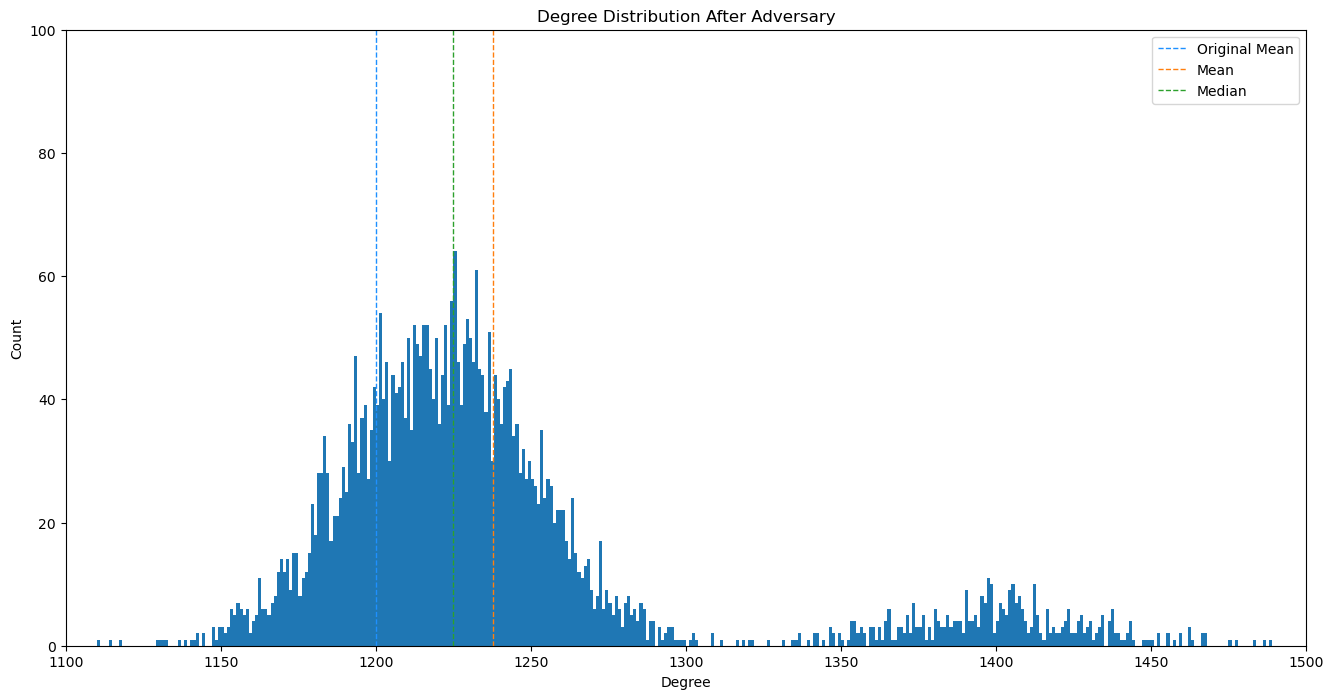
\includegraphics[height=0.35\linewidth]{img/MAM_intuit.png}
    \caption{\((n-1)p\) plotted along with the mean and median of the altered distribution}
    \label{fig:mean-vs-median}
\end{figure}

The resulting algorithm for the Mean-Adjusted median is described in Algorithm \ref{alg:mean-adjusted median}.

\begin{algorithm}
\caption{Mean-Adjusted Median}\label{alg:mean-adjusted median}
\begin{algorithmic}
\Require Laplacian matrix L, epsilon $\epsilon$
\State $D \gets $Degrees of vertices using $L$
\State $\bar{p} \gets $ normalized mean 
\State $\tilde{p} \gets$ normalized median
\State \Return $\frac{(2-\epsilon)\tilde{p} - \bar{p}}{1-\epsilon}$
\end{algorithmic}
\end{algorithm}

For the empirical and theoretical results presented in this paper, we adopt the (\(q,\epsilon\))-oblivious adversary.

\begin{defin}
    \label{(q, epsilon)-Adversary}
    Let \( G \sim G(n,p)\). The {\bf $(q,\eps)$-oblivious adversary} randomly selects a subset \(B\subset V\) of corrupted vertices with \(|B| = \eps n\) and rewires edges adjacent to \( B \) according to a new edge probability \( q \), such that:
    
    \[
    \mathbb{P}((u, v) \in E') =
    \begin{cases} 
    q, & \text{if } u \in B \text{ or } v \in B, \\
    1, & \text{if }  u,v\notin B \text{ and } (u,v) \in E\\
    0, & \text{if } u,v\notin B \text{ and } (u,v) \notin E\\
    \end{cases}
    \]
    where \(E'\) is the edge set of \(\mathcal{A}(G)\).
\end{defin}

While the \((q, \epsilon)\)-adversary is not as powerful as the \(\epsilon\)-omniscient adversary, it can still significantly alter the graph's structure and simulate major shifts in connectivity similar to those caused by the \(\epsilon\)-omniscient adversary. Therefore, evaluating whether the Mean-Adjusted Median algorithm can accurately estimate the edge probability \(p\) under the influence of a \((q, \epsilon)\)-adversary serves as a robust test of the algorithm's resilience and offers a valuable direction for further study.

\begin{thm}
  \label{theorem: mean-adjusted-median}
  Given a graph perturbed by a (\(q,\epsilon\))-adversary with $\epsilon < 0.5$, the Mean-Adjusted Median algorithm has a runtime of \(O(n)\) and a guaranteed error of 
  \[|p - \hat{p}| \leq O\left(\frac{1}{\sqrt[4]{n}}\right)\] with probability at least $1-\frac{1}{\sqrt n}$.
\end{thm}
\begin{proof}
Let $D'$ be the degree distribution of the perturbed graph. We then calculate the normalized mean \(\bar{p'}\) and the normalized median \(\tilde{p'}\) of the $D'$ by taking the mean and median of \(D'\) and dividing by \(n-1\). Both the mean and median can be computed in \(O(n)\) time. Finally, we run an \(O(1)\) operation to return the mean-adjusted median. The algorithm has a runtime of \(O(n)\). 

The error of the algorithm is given by the absolute difference between the mean-adjusted median and the true edge probability \(p\). We start by examining the degrees of the vertices in the graph, which are directly proportional to the edge probability \(p\) of the graph. 

Let \(\tilde{d'}\) and \(\bar{d'}\) be the median and mean of $D'$. Let $\eta = p - q$, $\hat d := \frac{(2-\eps)\tilde{d'} - \bar{d'}}{1-\eps}$, and $\hat p := \frac{\hat d}{n-1}$.

By Lemma \ref{lem: exp p_hat} in the Appendix \ref{proofs for mean-adjusted median algorithm}, $\hat p$ is a random variable such that $\ee[\hat p] \approx p - \frac{\epsilon\eta + (2\eps - \eps^2)\frac{\mathrm{Sign}(\eta)}{2a}}{(1-\eps)(n-1)}$ where $$a = \frac{1-\eps}{\sqrt{2\pi}\sigma_X} + \frac{\eps}{\sqrt{2\pi}\sigma_Y}e^{-\frac{(\mu_X-\mu_Y)^2}{2\sigma_Y^2}}.$$ Here, \begin{align*}
    \mu_X &= ((1-\eps)n-1)p + \eps nq;\\
    \sigma_X^2 &= ((1-\eps)n-1)p(1-p) + \eps nq(1-q);\\
    \mu_Y &= (n-1)q;\\
    \sigma_Y^2 &= (n-1)q(1-q).
\end{align*}

Then we observe that $$p - \hat p = (p - \ee[\hat p]) + (\ee[\hat p] - \hat p) \approx (\ee[\hat p] -\hat p) + \frac{\epsilon\eta + (2\eps - \eps^2)\frac{\mathrm{Sign}(\eta)}{2a}}{(1-\eps)(n-1)}.$$ By the triangle inequality, $$|p - \hat p| \leq |\ee[\hat p] - \hat p| + \left|\frac{\eps\eta + (2\eps -\eps^2)\frac{\mathrm{Sign}(\eta)}{2a}}{(1-\eps)(n-1)}\right|\leq |\ee[\hat p] -\hat p| + \frac{\eps + \frac{2\eps-\eps^2}{2a}}{(1-\eps)(n-1)}.$$

In the proof of Lemma \ref{lem: var p_hat}, we showed that $a \geq \frac{1}{2\sqrt{\pi n}}$, which implies $\frac{1}{a}\in[0, 2\sqrt{\pi n}]$. As a result, $$|p-\hat p| \leq |\ee[\hat p] -\hat p| + \frac{\eps + (2\eps-\eps^2)\sqrt{\pi n}}{(1-\eps)(n-1)} \leq |\ee[\hat p] -\hat p| + \frac{8\eps}{\sqrt n}$$ Moreover, as $n\to\infty$, the bias $\frac{\epsilon\eta + (2\eps - \eps^2)\frac{\mathrm{Sign}(\eta)}{2a}}{(1-\eps)(n-1)} \in \left[\frac{\eps\eta}{(1-\eps)(n-1)}, \frac{\eps\eta + (2\eps - \eps^2)\sqrt{\pi n}}{(1-\eps)(n-1)}\right]$ goes to zero. Thus, the mean of $\hat p$ approaches $p$.

By Lemma \ref{lem: var p_hat}, we have $\Var(\hat p) \leq 64\frac{1 + \sqrt{n} + n}{n^2} \leq \frac{256}{n}$ since $n\geq 1$. Using Chebyshev's inequality, for any $\delta > 0$, $$\Pr(|\hat p-\ee[\hat p]\geq \delta)\leq \frac{\Var(\hat p)}{\delta^2} \leq \frac{256}{\delta^2n}.$$ Hence, with probability at least $1 - \frac{256}{\delta^2 n}$, $$|p-\hat p| \leq |\ee[\hat p]-\hat p| + \frac{8\eps}{\sqrt{n}} \leq \delta + \frac{8\eps}{\sqrt{n}}.$$ Letting $\delta = \frac{16}{\sqrt[4]{n}}$, we conclude that with probability at least $1-\frac{1}{\sqrt{n}}$, $$|p -\hat p| \leq \frac{16}{\sqrt[4]{n}} + \frac{8\eps}{\sqrt{n}}\leq O\left(\frac{1}{\sqrt[4]{n}}\right)$$ as desired.


% This implies that the standard deviation of $\hat p$ is at most $\frac{16}{\sqrt{n}}$. As $n$ grows large, the standard deviation shrinks. In other words, $\hat p$ is not only shifting its mean closer to $p$ but also becoming more tightly concentrated around its mean.
\end{proof}



\section{Bias-Corrected Mean-Adjusted Median}

In the previous section, letting $\hat{p}$ denote the output of the Mean-Adjusted Median algorithm, we showed that the expected value of $\hat{p}$ is approximately $$\mathbb{E}[\hat{p}] \approx p - \frac{\eps\eta + (2\eta - \eta^2)\frac{\mathrm{Sign}(\eta)}{2a}}{(1-\eps)(n-1)}.$$ Although the bias diminishes as $n$ increases, we aim to remove this bias entirely. However, the bias term depends on $\eps, p, q,$ and $n$. While $\eps$ and $n$ are known, $p$ and $q$ are unknown quantities.

Due to the relative weakness of the $(q, \eps)$-oblivious adversary, we can compute $\mathbb{E}[\bar{p'}]$ as a function of $p, q, \eps,$ and $n$. By Lemma \ref{lem: exp bar d'}, we have $$\mathbb{E}[\bar{p'}] = \frac{\mathbb{E}[\bar{d'}]}{n-1} = p - 2\eps\eta + \eps^2\eta - \frac{\eta(\eps-\eps^2)}{n-1}.$$ Rewriting this, $$\mathbb{E}[\bar{p'}] = p\left(1 - 2\eps + \eps^2 - \frac{\eps-\eps^2}{n-1}\right) + q\left(2\eps - \eps^2 + \frac{\eps-\eps^2}{n-1}\right).$$

We can then express $q$ as a function of $p, \eps, \mathbb{E}[\bar{p'}],$ and $n$: $$q = \frac{\mathbb{E}[\bar{p'}] - p\left(1 - 2\eps + \eps^2 - \frac{\eps-\eps^2}{n-1}\right)}{2\eps - \eps^2 + \frac{\eps-\eps^2}{n-1}} = p + \frac{\ee[\bar{p'}] - p}{2\eps - \eps^2 + \frac{\eps-\eps^2}{n-1}}.$$

For large $n$, the sample mean, $\bar{p'}$, which we can compute given the perturbed graph, closely approximates $\mathbb{E}[\bar{p'}]$, and $\hat{p}$ is a good estimation of $p$ with high probability as established in Theorem \ref{theorem: mean-adjusted-median}, $\hat{p}$. Thus, we define an estimator for $q$: $$\hat{q} = \hat p + \frac{\bar{p'} - \hat p}{2\eps - \eps^2 + \frac{\eps-\eps^2}{n-1}}.$$ Using $\hat p, \hat{q},\eps$, and $n$, we estimate $\eta$ as $\hat{\eta} := \hat{p} - \hat{q}$ and $a$ by $\hat{a}$. Using $\hat\eta$ and $\hat a$, we are then able to estimate the bias term $\frac{\eps\eta + (2\eta - \eta^2)\frac{\mathrm{Sign}(\eta)}{2a}}{(1-\eps)(n-1)}.$ Finally, instead of returning $\hat{p}$, we return the adjusted estimator $$\hat{p}^* := \hat{p} + \frac{\eps\hat{\eta} + (2\hat{\eta} - \hat{\eta}^2)\frac{\mathrm{Sign}(\hat{\eta})}{2\hat{a}}}{(1-\eps)(n-1)}.$$

The resulting algorithm for the Bias-Corrected Mean-Adjusted Median is described in Algorithm \ref{alg:bias-corrected mean-adjusted median}.
\begin{algorithm}
\caption{Bias-Corrected Mean-Adjusted Median}\label{alg:bias-corrected mean-adjusted median}
\begin{algorithmic}
\Require Laplacian matrix $L$, epsilon $\epsilon$
\State $D \gets $Degrees of vertices in $L$
\State $\bar{p'} \gets $ normalized mean 
\State $\hat p \gets \Call{Mean-Adjusted-Median}{L, \eps}$
\State $\hat q \gets \hat p + \frac{\bar{p'} - \hat p}{2\eps - \eps^2+\frac{\eps-\eps^2}{n-1}}$
\State $\hat\eta, \hat a \gets$ estimation of $\eta, a$ using $\hat p, \hat q, \eps, n$
% \State $y \gets \frac{1}{1 - \epsilon} |\bar{p} - \tilde{p}|$
% \If {$\bar{p} \leq \tilde{p}$}
%     \State \Return $\tilde{p} - y$
% \Else
%     \State \Return $\bar{p} - y$
% \EndIf
\State \Return $\hat p + \frac{\eps\hat\eta + (2\hat\eta - \hat\eta^2)\frac{\mathrm{Sign}(\hat\eta)}{2\hat a}}{(1-\eps)(n-1)}$
\end{algorithmic}
\end{algorithm}

While $\hat{p}^*$ is not strictly unbiased due to the approximations, it is effective in reducing the bias. 

We empirically test the Bias-Corrected Mean-Adjusted Median algorithm and find that it consistently outperforms the original Mean-Adjusted Median algorithm, achieving improved accuracy in estimating $p$. The analysis can be found in Section \ref{results}.


% \subsection{Empirical Results}

% 


\section{Variance-Based Filtering}
In this section, we propose a variance-based algorithm for robustly estimating the parameter $p$ on an adversarially corrupted graph \(\mathcal{A}(G)\). The key idea is that the variance of the degree distribution of the vertices in \(\mathcal{A}(G)\) can provide insight into which vertices have been corrupted. Thus, we can study the difference in variance between the perturbed sample graph and the expected variance, assuming a binomial distribution. Even in an adversarially perturbed graph, the degree distribution of the subgraph consisting of the uncorrupted vertices follows a binomial distribution. Therefore, the observed variance of such a subgraph should equal the theoretical variance. However, the degree distribution of the vertices in \(\mathcal{A}(G)\) may not follow a binomial distribution. The variance-based filtering algorithm seeks to uncover this subgraph of uncorrupted vertices by minimizing the difference in the theoretical variance and the observed variance. Formally, we define $s^2 = \frac{1}{n-1} \sum_{v \in V}{(\deg(v) - \bar{d})^2}$ where $V$ denotes the set of vertices. Similarly, we define $\hat{\sigma}^2 = n \hat{p} (1 - \hat{p})$ where $\hat{p}$ denotes the mean of the degree distribution assuming a binomial distribution. On an unperturbed graph, since the degrees of the vertices roughly follow a binomial distribution, $\left| s^2 - \hat{\sigma}^2 \right|$ will be small, with high probability. We exploit this fact in Algorithm \ref{alg:variance algorithm}.

\begin{algorithm}
\caption{Variance Algorithm}\label{alg:variance algorithm}
\begin{algorithmic}
\Require Laplacian matrix $L$, epsilon $\epsilon$
\State $n \gets $number of vertices
\State $V \gets $set of all vertices
\While{$t = 0, t < \epsilon n$}
\For{\text{vertex $v$ in V}}
\State Compute subgraph after removing $v$ using $L$
\State Compute and store $\left| s^2_{G_{(V \setminus \{v\})}} - \hat{\sigma}^2_{G_{(V \setminus \{v\})}} \right|$ for the given vertex $v$
\EndFor
\State $x \gets \max_{v \in V} \left| s^2_{G_{(V \setminus \{v\})}} - \hat{\sigma}^2_{G_{(V \setminus \{v\})}} \right|$
\State $V \gets V \setminus x$
\EndWhile
\end{algorithmic}
\end{algorithm}

This iterative algorithm seeks to remove vertices that cause the greatest difference to the variance. Assuming we start with a graph \(G \sim G(n, p)\), we remove the vertex that maximizes: $$\max_{v \in V} \left| s^2_{G_{(V \setminus \{v\})}} - \hat{\sigma}^2_{G_{(V \setminus \{v\})}} \right|.$$ Since we know that in an unperturbed graph, $|s^2 - \hat{\sigma}^2|$ is small with high probability, removing the vertex that causes the greatest deviation with this term would enable us to reduce the difference in the observed and expected variance, ultimately converging on a set of vertices where this term is minimized. It is important to note, though, that the vertices that minimize this difference may not always converge to the true set of uncorrupted vertices. We implement this removal process $\eps$$n$ times in order to remove an $\eps$-fraction of the vertices, simulating removing the corrupted vertices. However, since we minimize the difference between the variances, the subgraph that remains has a degree distribution that is the best candidate among all subgraphs to follow a binomial distribution after $\eps$$n$ vertex removals. The time complexity of this variance-based filtering algorithm is $O(\eps n^3)$ since we iterate $\eps$$n$ times and in each iteration, we simulate removing every vertex, which takes $O(n)$ time, and calculating the variance on this new subgraph, also $O(n)$ time. 

\section{Results} \label{results}
To evaluate these different models on estimating the parameter $p$, we compare the mean-squared error across the methods on the $\left(q, \eps \right)$-adversary. Since the spectral method is bounded by $\eps < 1 / 60$, we evaluate the experiments in Figure \ref{fig:result3} with an $\eps = 0.01$ and the experiments in Figures \ref{fig:result1}, \ref{fig:result2}, \ref{fig:result4} with an $\eps = 0.1$ 
\cite{acharya2022robustestimationrandomgraphs}. For each data point, we run each method on 20 trials and take the average of the estimates for a holistic measure of the mean-squared error.

Figure \ref{fig:result1} displays a comparison of the mean-squared error across six different methods: the naive mean, naive median, prune-then-mean, prune-then-median, mean-adjusted median, and bias-corrected mean-adjusted median algorithms. From Figure \ref{fig:result1}, we observe that as the number of vertices in the \erdos graph increases, the empirical error of the naive mean and median algorithms remains fairly stable. This is because the error of these algorithms scales with regards to $\eps$ and is not correlated with $n$ \cite{acharya2022robustestimationrandomgraphs}.

Figure \ref{fig:result2} shows a more focused depiction of the more robust mean and median-based algorithms from \ref{fig:result1}. Empirically, all of these algorithms scale inversely with respect to $n$ since the mean-squared error decreases as the number of vertices $n$ increases. We notice the Bias-Corrected Mean-Adjusted Median algorithm performs significantly better than the plain Mean-Adjusted Median algorithm, empirically demonstrating that we can successfully remove the bias term from Mean-Adjusted Median algorithm.

Figure \ref{fig:result3} compares the Mean-Adjusted Median algorithms with the Spectral Method and the Variance-Based filtering method. Due to computational reasons, we limit running the Spectral method on graphs with less than 500 nodes. We notice that the Spectral Method and the Variance-based Filtering method perform better than the Mean-Adjusted Median method. 

Finally, figure \ref{fig:result4} displays all of the datapoints for the variance-based filtering algorithm with the 20 trials shown for a given $n$. The line plot displayed takes the mean error of these 20 trials to illustrate a general trend in the error as the number of vertices increases. It is important to note that the error in this figure is the absolute error, rather than the mean-squared error.

\begin{table}[ht]
    \centering
    \begin{tabular}{lcc}
        \textbf{Methods} & \textbf{Runtime} & \textbf{Authors}\\
        \hline
        {Mean/Median} & O(n) & Acharya et al.\\
        {Prune then Mean/Median} & $O(n\log(\eps n))$ & Acharya et al.\\
        {Spectral Method} & $\tilde{O}\left(\eps n^3\right)$ & Acharya et al.\\
        {Mean-Adjusted Median} & $O(n)$ & Lee et al.\\
        {Bias-Corrected Mean-Adjusted Median} & $O(n)$ & Lee et al.\\
        {Variance Method} & $O(\eps n^3)$ & Lee et al.\\
    \end{tabular}
    % \caption{Runtimes of the algorithms mentioned in this paper}
    \label{tab:runtimes}
\end{table}

\begin{figure}[ht]
    \centering
    % First row with two figures
    \begin{minipage}{0.45\textwidth}
        \centering
        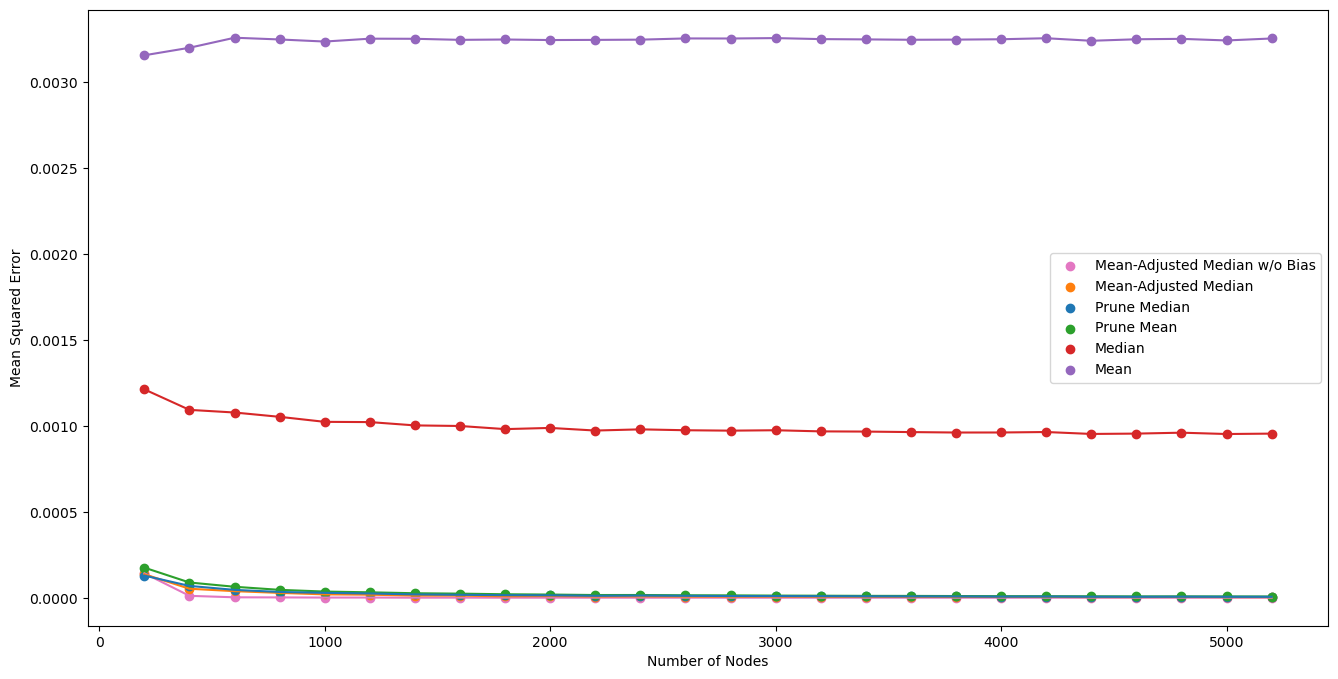
\includegraphics[width=\linewidth]{img/emperic.png}
        \caption{$\eps=0.1$, $p = 0.3$, $q = 0.6$}
        \label{fig:result1}
    \end{minipage} \hfill
    \begin{minipage}{0.45\textwidth}
        \centering
        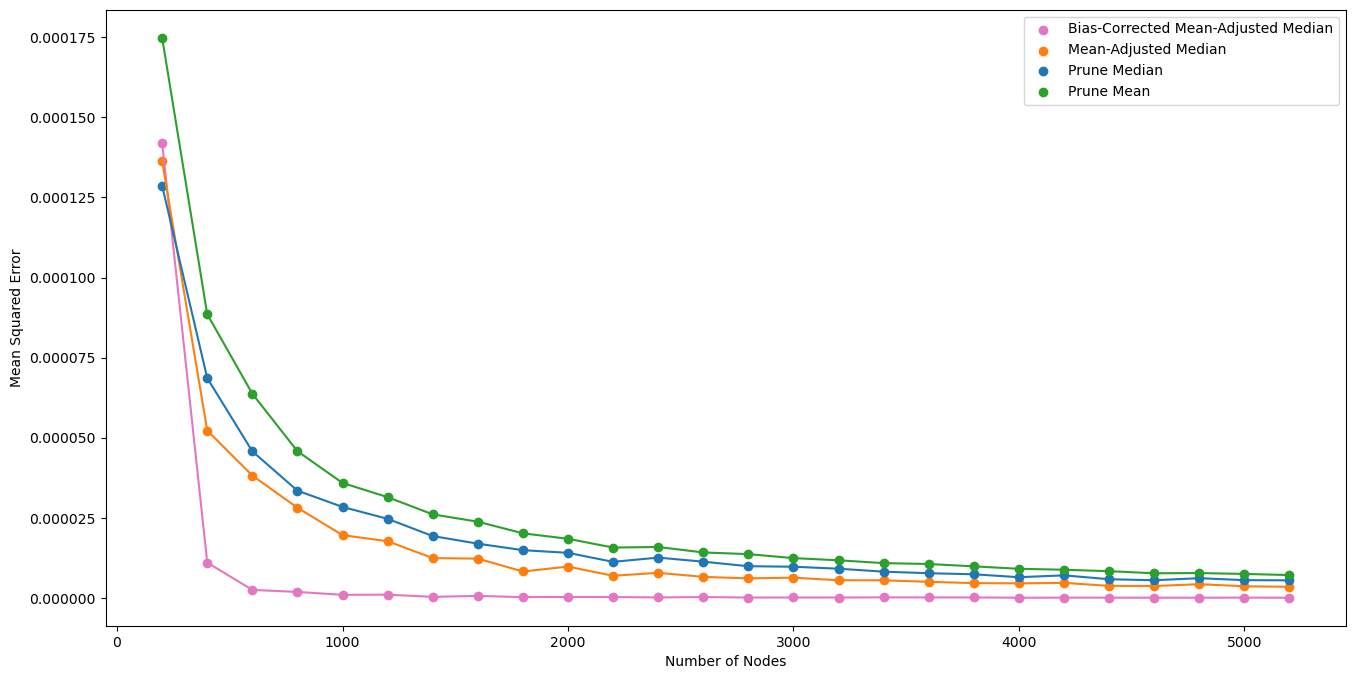
\includegraphics[width=\linewidth]{img/emperic2.png}
        \caption{$\eps = 0.1$, $p = 0.3$, $q = 0.6$}
        \label{fig:result2}
    \end{minipage}
\end{figure}

\begin{figure}[ht]
    % Second row with two figures
    \begin{minipage}{0.45\textwidth}
        \centering
        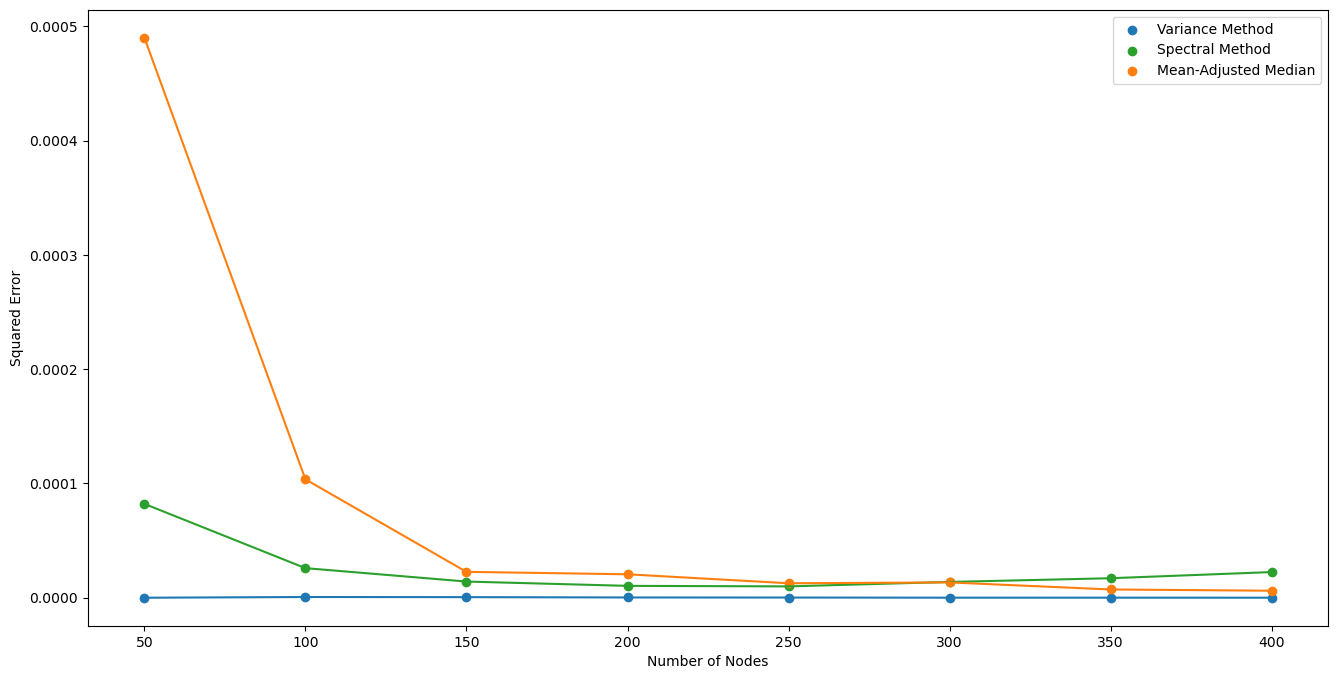
\includegraphics[width=\linewidth]{img/emperic3.png}
        \caption{$\eps = 0.01$, $p = 0.3$, $q = 0.6$}
        \label{fig:result3}
    \end{minipage} \hfill
    \begin{minipage}{0.45\textwidth}
        \centering
        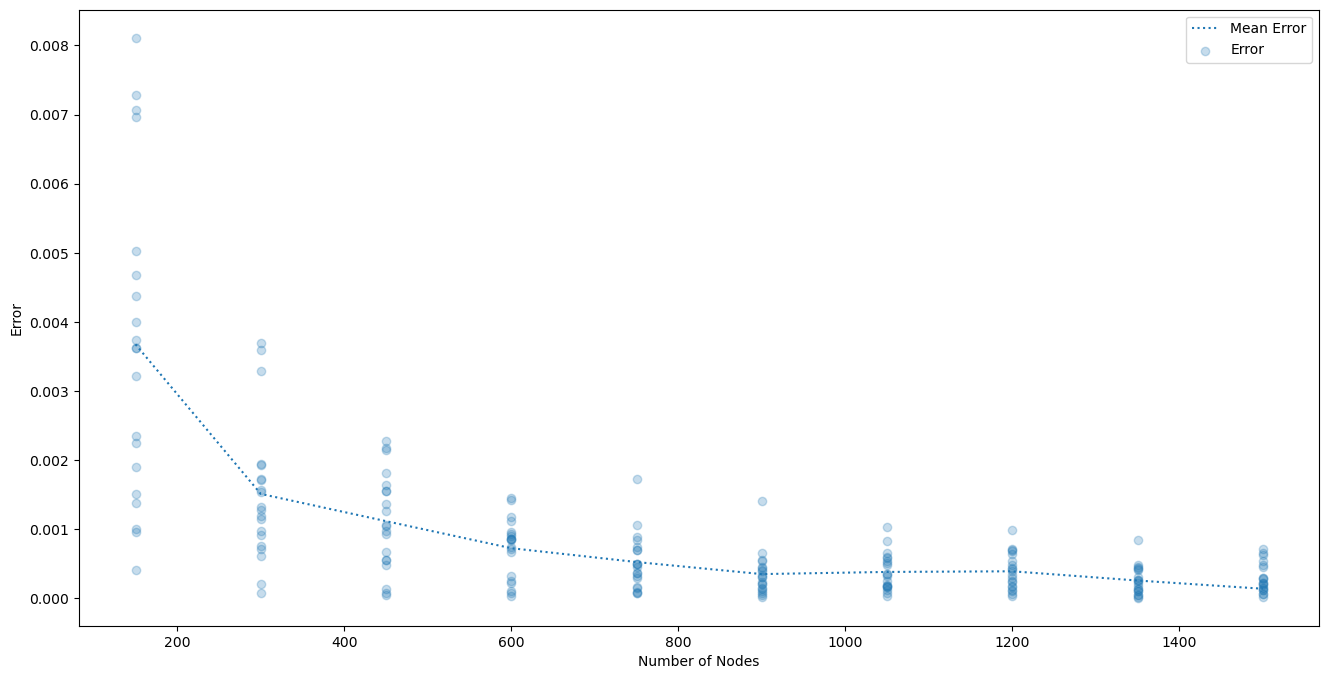
\includegraphics[width=\linewidth]{img/emperic4.png}
        \caption{Each dot represents a trial; $\eps = 0.1$, $p = 0.3$, $q = 0.6$}
        \label{fig:result4}
    \end{minipage}
\end{figure}


\section{Conclusion}
In this work, we introduced a novel adversarial framework, the \((q, \eps)\)-adversary model, and proposed three algorithms for robust estimation of the edge probability \(p\) in adversarially perturbed Erdős-Rényi random graphs: the Mean-Adjusted Median, Bias-Corrected Mean-Adjusted Median, and Variance-Based Filtering algorithms. By extending the adversarial models proposed in prior research, our models tackle adversarially corrupted graphs using the mean, median, and the variance.

The theoretical analysis in Theorem \ref{theorem: mean-adjusted-median} establishes that the Mean-Adjusted Median algorithm guarantees a bounded error of \(O\left(\frac{1}{\sqrt[4]{n}}\right)\) with high probability, while maintaining an efficient runtime of \(O(n)\). This gurantee highlights that on the $(q,\eps)$-oblivious adversary, the Mean-Adjusted Median algorithm outperforms the naive mean and median algorithms. The Bias-Corrected Mean-Adjusted Median builds on this foundation by addressing bias, leading to improved accuracy in empirical evaluations. Additionally, the Variance-Based Filtering algorithm effectively identifies corrupted vertices, albeit with a higher computational cost of \(O(\varepsilon n^3)\). 

We present empirical evaluations of the mean-squared errors and runtime comparisons of these algorithms, focusing on their performance against the \((q, \varepsilon)\)-adversary. Our results confirm the theoretical upper bound for the Mean-Adjusted Median, showing \(\left| p - \hat{p} \right| \leq O(1/\sqrt[4]{n})\), while highlighting the practical advantages of our proposed methods over baseline techniques. Furthermore, the empirical results demonstrate that these methods outperform existing techniques in practice, such as prune-then-mean/median and the spectral method by Acharya et al., in both error and runtime efficiency when applied to \((q, \varepsilon)\)-oblivious adversaries.

Our findings provide valuable insights into designing robust algorithms for graph parameter estimation under adversarial perturbations. Future work could focus on extending the theoretical guarantees of the proposed algorithms to \(\varepsilon\)-omniscient adversaries. Appendix \ref{proofs for variance algorithm} includes proofs of lemmas that could serve as a foundation for establishing these guarantees. Another promising direction involves investigating applications of these methods in real-world networks.

\textcolor{white}{Heon is the MVP}

{\small
\bibliographystyle{ieee}
\bibliography{egbib}
}

\newpage
\appendix
\section{Proofs for Mean-Adjusted Median Algorithm} \label{proofs for mean-adjusted median algorithm}
In this section, let $D'$ be the degree distribution of the graph perturbed by the $(q,\eps)$-oblivious adversary. Let $\bar{d'}$ and $\tilde{d'}$ be the mean and median of $D'$, respectively.
\begin{lem} \label{lem: exp bar d'}
$\ee[\bar{d'}] = (n-1)p + \eps(1-2n)\eta + \eps^2n\eta$ where $\eta := p-q$.
\end{lem}
\begin{proof}
By definition, for $v\in R'$, $$\ee[\deg(v)] = \ee\left[\sum_{u\in R', u\neq v}X_{uv} + \sum_{u\in S'}X_{uv}\right] =((1-\eps)n-1)p + \eps nq$$ and for $v\in S'$, $$\ee[\deg(v)] = (n-1)q.$$ Therefore, \begin{align*}
    \ee[\bar{d'}] &=  \frac{1}{n}\left(\sum_{v\in R'}\ee[\deg(v)] + \sum_{v\in S'}\ee[\deg(v)] \right)\\
    &= \frac{1}{n}\left(\sum_{v\in R'}(((1-\eps)n -1)p + \eps nq) + \sum_{v\in S'}(n-1)q \right)\\
    &= (n-1)p + \eps(1-2n)\eta + \eps^2n\eta.\qedhere
\end{align*}
\end{proof}

Letting $D' = \{D_1', \dots, D_n'\}$, let $D_1',\dots, D_{(1-\eps)n}'$ be the degrees of the uncorrupted vertices and $D_{(1-\eps)n}',\dots, D_n'$ be the degrees of the corrupted vertices. 

Let $X = U + W$ where $U \sim \mathrm{Binomial}(\eps n, q)$ and $W\sim\mathrm{Binomial}((1-\eps)n-1, p)$, and $Y\sim\mathrm{Binomial}(n-1, q)$. Then the uncorrupted sample is drawn from the distribution of $X$ and the corrupted sample is drawn from the distribution of $Y$. As $n$ grows large, the dependence of pairwise sample asymptotically approaches 0, so we may assume that the samples are drawn iid from $X$ and $Y$, respectively.

We now observe that for large $n$, $X$ and $Y$ can be approximated using the normal distribution due to the Central Limit Theorem. Hence, $$X\sim N(\mu_X, \sigma_X^2), Y \sim N(\mu_Y, \sigma_Y^2)$$ where \begin{align*}
    \mu_X &= ((1-\eps)n-1)p + \eps nq;\\
    \sigma_X^2 &= ((1-\eps)n-1)p(1-p) + \eps nq(1-q);\\
    \mu_Y &= (n-1)q;\\
    \sigma_Y^2 &= (n-1)q(1-q).
\end{align*} For the remainder of our analysis, we proceed under this simplifying assumption.

Thus, we have a sample of size $n$ drawn from the mixture distribution $$Z :=\begin{cases}
    X &\text{w.p. }(1-\eps)\\
    Y &\text{w.p. }\eps.
\end{cases}$$

\begin{lem} \label{lem: var bar d'}
$\Var(\bar{d'}) = \frac{(1-\eps)\sigma_X^2 + \eps\sigma_Y^2 + \eps(1-\eps)(\mu_X - \mu_Y)^2}{n}$
\end{lem}
\begin{proof}
We have $$\Var(\bar{d'}) = \frac{\Var(Z)}{n} = \frac{(1-\eps)\Var(X) + \eps\Var(Y) + \eps(1-\eps)(\mu_X - \mu_Y)^2}{n}$$ as desired.
\end{proof}

\begin{lem} \label{lem: exp tilde d'}
$$\ee[\tilde{d'}] \approx \mu_X - \eps\frac{\mathrm{Sign}(\eta)}{2a}$$ where $a := (1-\eps)/\sqrt{2\pi\sigma_X^2} + \eps \frac{\eps}{\sqrt{2\pi}\sigma_Y}e^{-\frac{(\mu_X-\mu_Y)^2}{2\sigma_Y^2}}$.
\end{lem}
\begin{proof}
We know that the expected median $\ee[\tilde{d'}]$ of $D'$ satisfies: \begin{equation}\label{eq:med1}
    (1 - \eps) F_X(\ee[\tilde{d'}]) + \eps F_Y(\ee[\tilde{d'}]) = 0.5
\end{equation} where $F_X$ and $F_Y$ are the CDFs of $X$ and $Y$, respectively.

We now approximate the CDFs using a Taylor expansion. Since $\eps$ is small, we linearize around the median of $X$. Since $X$ is normal, the median of $X$ is $\mu_X$. Letting $\Delta = \ee[\tilde{d'}] -\mu_X$, then $$F_X(\ee[\tilde{d'}]) = 0.5 + \sum_{k=0}^\infty f_X^{(k)}(\mu_X)\Delta^k$$ and 
$$F_Y(\ee[\tilde{d'}]) = F_Y(\mu_X) + f_Y(\mu_X)\Delta + O(\Delta^2) \approx  F_Y(\mu_X) + f_Y(\mu_X)\Delta$$ where $f_X$ and $f_Y$ are the PDFs of $X$ and $Y$. Since $X$ is normal, we know that the $f^{(k)}(\mu_X) = 0$ for $k > 0$. Hence, $$F_X(\ee[\tilde{d'}]) = 0.5 + \frac{1}{\sqrt{2\pi \sigma_X^2}}\Delta.$$

Substituting the expansion into Equation \ref{eq:med1}, we know $$(1-\eps)\left(0.5 + \frac{\Delta}{\sqrt{2\pi\sigma_X^2}}\right) + \eps\left(F_Y(\mu_X) + f_Y(\mu_X)\Delta\right) = 0.5.$$ Simplifying and solving for $\Delta$, we have $$\Delta = -\epsilon\frac{F_Y(\mu_X) - 0.5}{a}$$ where $$a := (1-\eps)/\sqrt{2\pi\sigma_X^2} + \eps f_Y(\mu_X) = \frac{1-\eps}{\sqrt{2\pi\sigma_X^2}} + \frac{\eps}{\sqrt{2\pi}\sigma_Y}e^{-\frac{(\mu_X-\mu_Y)^2}{2\sigma_Y^2}},$$ implying that \begin{equation}\label{eq:med2}
    \ee[\tilde{d'}] \approx \mu_X - \epsilon\frac{F_Y(\mu_X) - 0.5}{a}.
\end{equation}

We now express $F_Y(\mu_X) - 0.5$ in terms of standard normal variables. Letting $$z = \frac{\mu_X - \mu_Y}{\sigma_Y} = \frac{(n(1-\eps) - 1)\eta}{\sqrt{n q (1 - q)}},$$ then $F_Y(\mu_X) = \Phi(z)$ where $\Phi$ is the standard normal CDF. Then $$F_Y(\mu_X) - 0.5 = \Phi(z) -0.5.$$

Substituting back into Equation \ref{eq:med2}, then $\ee[\tilde{d'}]$ is $$\ee[\tilde{d'}] \approx \mu_X - \epsilon\frac{\Phi(z) - 0.5}{a}.$$ 

We now observe that assuming $q\in (0,1)$, $z = \frac{(n(1 - \eps) - 1)\eta}{\sqrt{nq(1-q)}} \approx \mathrm{Sign}(\eta)C\sqrt{n}$ for some constant $C> 0$. For $z \geq 3$, we know $\Phi(z) \in [0.99, 1]$, and for $z \leq 3$, we know that $\Phi(z) \in [0, 0.01]$. Consequently, $\Phi(z) - 0.5 \approx \begin{cases}
    0.5 &\text{if }p>q\\
    -0.5 &\text{if }p<q\\
    0 &\text{if }p=q,
\end{cases}$ with the approximation being tighter for increasing $n$. Then, $$\Phi(z) - 0.5 \approx \frac{\mathrm{Sign}(\eta)}{2}.$$ Therefore, $$\ee[\tilde{d'}]\approx \mu_X - \eps\frac{\Phi(z) - 0.5}{a} \approx \mu_X - \eps\frac{\mathrm{Sign}(\eta)}{2a}$$ as desired.
\end{proof}

\begin{lem} \label{lem: var tilde d'}
$$\Var(\tilde{d'}) \approx \frac{1}{4na^2}$$ where $a = (1-\eps)/\sqrt{2\pi\sigma_X^2} + \eps f_Y(\mu_X)$.
\end{lem}
\begin{proof}
Again, assuming that our samples are drawn i.i.d., for large $n$, the sample median of i.i.d. draws from a continuous distribution with PDF $f_Z$ at its median $\ee[\tilde{d'}]$ (where $F_Z(\ee[\tilde{d'}])=0.5$) has an asymptotic normal distribution. Using the delta method on the central limit theorem, we know that $$\operatorname{Var}\left(\tilde{d}^{\prime}\right) \approx \frac{1}{4 n f_Z(\ee[\tilde{d'}])^2} \approx \frac{1}{4 n f_Z(\mu_X)^2} = \frac{1}{4na^2}.$$
\end{proof}

We claim that $\hat p := \frac{\hat d}{n-1}$ where $\hat d := \frac{(2-\eps)\tilde{d'} - \bar{d'}}{1-\eps}$ is a good estimator of $p$. We first show that the expected value of $\hat p$ is close to $p$ and that the variance is also small.

\begin{lem}\label{lem: exp p_hat}
$\ee[\hat p] \approx p - \frac{\eps\eta + (2\eps-\eps^2)\frac{\mathrm{Sign}(\eta)}{2a}}{(1-\eps)(n-1)}.$
\end{lem}
\begin{proof}
We first find $\ee[\hat d]$. By Lemmas \ref{lem: exp bar d'} and \ref{lem: exp tilde d'}, we have \begin{align*}
    \ee[\hat d] &= \ee\left[\frac{(2-\eps)\tilde{d'} - \bar{d'}}{1-\eps}\right]\\
    &= \frac{(2-\eps)\ee[\tilde{d'}] - \ee[\bar{d'}]}{1-\eps}\\
    &\approx \frac{(2-\eps)\left[\mu_X - \eps\frac{\mathrm{Sign}(\eta)}{2a}\right] - [(n-1)p + \eps(1-2n)\eta + \eps^2n\eta]}{1-\eps}\\
    &= (n-1)p - \frac{\eps\eta + (2\eps-\eps^2)\frac{\mathrm{Sign}(\eta)}{2a}}{1-\eps}.
\end{align*}

Because $\hat p :=\frac{\hat d}{n-1}$, then \begin{align*}
    \hat p &\approx \frac{(n-1)p - \frac{\eps\eta + (2\eps-\eps^2)\frac{\mathrm{Sign}(\eta)}{2a}}{1-\eps}}{n-1}\\
    &= p - \frac{\eps\eta + (2\eps-\eps^2)\frac{\mathrm{Sign}(\eta)}{2a}}{(1-\eps)(n-1)}
\end{align*} as desired.
\end{proof}

\begin{lem} \label{lem: var p_hat}
$\Var(\hat p) \leq 64\frac{1 + \sqrt{n} + n}{n^2}$.
\end{lem}
\begin{proof}
We first find bounds for $\sigma_X^2, \sigma_Y^2, (\mu_X - \mu_Y)^2$, and $a$. We know that $\eps\in[0, 0.5)$ and $p,q\in[0,1]$. Then $\eps(1-\eps), p(1-p), q(1-q) \leq 0.25$.

We then observe that \begin{align*}
    \sigma_X^2 &= ((1-\eps)n-1)p(1-p) + \eps nq(1-q) \\
    &\leq np(1-p) + \frac{nq(1-q)}{2}\\
    &\leq \frac{n}{4} + \frac{n}{8}\\
    &\leq \frac{n}{2}.
\end{align*} We also have that $$\sigma_Y^2 = (n-1)q(1-q)\leq \frac{n}{4}.$$ We then have that \begin{align*}
    (\mu_X - \mu_Y)^2 &= (((1-\eps)n-1)p + \eps nq - (n-1)q)^2\\
    &\leq (np + nq/2)^2\\
    &\leq 4n^2.
\end{align*} Finally, we observe that \begin{align*}
    a &= \frac{1-\eps}{\sqrt{2\pi}\sigma_X} + \frac{\eps}{\sqrt{2\pi}\sigma_Y}e^{-\frac{(\mu_X-\mu_Y)^2}{2\sigma_Y^2}}\\
    &\geq \frac{0.5}{\sqrt{2\pi}\sigma_X}\\
    [\sigma_X^2\leq n/2]&\geq \frac{1}{2\sqrt{2\pi}\sqrt{n/2}}\\
    &\geq \frac{1}{2\sqrt{\pi n}}.
\end{align*}

We now bound $\Var(\tilde{d'})$ and $\Var(\bar{d'})$. Using Lemma \ref{lem: var tilde d'} and $a\geq \frac{1}{2\sqrt{\pi n}}$, we observe that $$\Var(\tilde{d'}) = \frac{1}{4na^2} \leq \frac{1}{4n\left(\frac{1}{2\sqrt{\pi n}}\right)^2} = \pi.$$ Using Lemma \ref{lem: var bar d'} and our previously found bounds, we observe that \begin{align*}
    \Var(\bar{d'}) &= \frac{(1-\eps)\sigma_X^2 + \eps\sigma_Y^2 + \eps(1-\eps)(\mu_X-\mu_Y)^2}{n}\\
    &\leq \frac{n/2 + n/8 + n^2}{n}\\
    &\leq 1 + n\\
    &\leq 2n.
\end{align*}

We know that by the Cauchy-Schwarz inequality, $|\mathrm{Cov}(X, Y)| \leq \sqrt{\Var(X)\Var(Y)}$ for any random variables $X, Y$. Hence, \begin{align*}
    \Var(\hat d) &= \Var\left(\frac{(2-\eps)\tilde{d'} - \bar{d'}}{1-\eps}\right)\\
    &= \frac{1}{(1-\eps)^2}\Var\left((2-\eps)\tilde{d'} - \bar{d'}\right)\\
    &= \frac{\Var((2-\eps)\tilde{d'}) + \Var(\bar{d'}) + 2\mathrm{Cov}((2-\eps)\tilde{d'}, \bar{d'})}{(1-\eps)^2}\\
    &\leq \frac{\Var((2-\eps)\tilde{d'}) + \Var(\bar{d'}) + 2\sqrt{\Var((2-\eps)\tilde{d'}) \Var(\bar{d'})}}{(1-\eps)^2}\\
    &\leq \frac{(2-\eps)^2\pi + 2n + 2(2-\eps)\sqrt{2\pi n}}{(1-\eps)^2}\\
    &\leq 16\pi + 8n + 16\sqrt{2\pi n}\\
    &\leq 64(1 + \sqrt{n} + n).
\end{align*} As a result, we know that $$\Var(\hat p) = \Var\left(\frac{\hat d}{n-1}\right) = \frac{\Var(\hat d)}{(n-1)^2} \leq 64\frac{1 + \sqrt{n} + n}{n^2}$$ as desired.
\end{proof}

\section{Proofs for Variance Algorithm}\label{proofs for variance algorithm}
\begin{lem}
\label{lemma: p_F - p}
Let $F$ be the subgraph of uncorrupted vertices. Then $|p_F - p| \leq \frac{1}{\sqrt{n}}$ with probability at least $1- 2\exp{\left(-(1-\epsilon)^2n\right)}$.
\end{lem}

\begin{proof}
Let $N_F := |F| = {(1-\epsilon)n\choose 2}$. Since each of the $N_F$ edges of $F$ is included independently with probability $p$, the number of edges in $F$, $E_F$, follows a binomial distribution: $$E_F\sim\mathrm{Binomial}(N_F, p).$$ Then the empirical edge probability $$p_F = \frac{E_F}{N_F}.$$ Because $\mu:= \ee[E_F] = N_Fp$ and the binomial distribution is the sum of independent Bernoulli distributions, by the Hoeffding inequality, $$\Pr(|p_F - p| \geq t) = \Pr(|E_F - \mu|/N_F \geq t)\leq2\exp(-2N_Ft^2).$$ Letting $t := \frac{1}{\sqrt{n}},$ then \begin{align*}
    \Pr\left(|p_F - p| \geq \frac{1}{n}\right) &\leq 2\exp(-2N_F/n)\\
    &= 2\exp\left(-\frac{2(1-\epsilon)n((1-\epsilon)n - 1)}{2n}\right)\\
    &= 2\exp(-(1-\epsilon)((1-\epsilon)n - 1))\\
    &= 2\exp(-(1-\epsilon)^2n)\exp(1-\epsilon)\\
    &\leq 2\exp(-(1-\epsilon)^2n).
\end{align*} Therefore, $$\Pr\left(|p_F - p| \leq \frac{1}{n}\right) \geq 1- 2\exp(-(1-\epsilon)^2n)$$ as desired.
\end{proof}

\begin{lem}
Let $F$ be the subgraph of uncorrupted vertices. Then $|\hat\sigma_F^2 - \sigma_F^2| \leq O\left(\sqrt{n}\right)$ with probability at least $1-2\exp(-(1-\epsilon)^2n)$.
\end{lem}
\begin{proof}
By Lemma \ref{lemma: p_F - p}, \begin{align*}
    |\hat\sigma_F^2 - \sigma_F^2| &= ((1-\epsilon)n-1)|p_F(1-p_F) - p(1-p)|\\
    &\leq ((1-\epsilon)n-1)\left|\frac{\sqrt{n}-2p\sqrt n -1}{n}\right|\\
    &\leq n\left|\frac{\sqrt{n}-2p\sqrt n -1}{n}\right|\\
    &\leq \left|\sqrt{n}-2p\sqrt n -1\right|\\
    &\leq O(\sqrt{n})
\end{align*}
\end{proof}

% \begin{lem}
% Let $F$ be the subgraph of uncorrupted vertices. Then $|s_F^2-\sigma_F^2| \leq O\left(?\right)$ with probability at least ?.
% \end{lem}

% \begin{thm}
% Let $F$ be the subgraph of uncorrupted vertices. Then $|\hat\sigma_F^2 - s_F^2| \leq O\left(?\right)$ with probability at least ?.
% \end{thm}

% \begin{proof}

% \end{proof}
\end{document}


% Abstract
% Background:
% * Erdös-reyni
%     * Definition
%     * Applications
% * Why this is hard (i.e. why standard robust estimators don’t work)
%     * Uncorrupted vertices are slightly corrupted
%     * Error of Mean
%     * Error of Median
% Related work:
% * Robust Estimation for Random Graphs
%     * Prune + Mean/Median
%     * Spectral Algorithm
% Notation:
% * G(n, p) - Random graph with n vertices and probability p
% * \mathcal{A}(G) - Adjacency matrix
% * [n] = \{1,…,n\} - vertex set
% * \sigma - population variance
% * s - sample variance
% Our work:
% * Problem statement - (q, epsilon)-adversary
% * Mean-Median
%     * Proof
% * Inefficient Coarse Estimator
% * Variance method
